\documentclass[11pt, a4paper, english]{NTNUoving}
\usepackage[utf8]{inputenc}
\usepackage[T1]{fontenc}
\usepackage{float}
\usepackage{enumitem}
\usepackage{csquotes}
\usepackage{algorithm}
\usepackage{algorithmic}
\usepackage{listings}
\usepackage{listings}
\usepackage{color}
\usepackage{biblatex}
\usepackage{hyperref}
\ovingnr{6}    % Nummer på innlevering
\semester{Spring 2021}
\fag{Optimization and Control \\ TTK4135}
\institutt{Department for Engineering Cybernetics}

\definecolor{mygreen}{RGB}{28,172,0} % color values Red, Green, Blue
\definecolor{mylilas}{RGB}{170,55,241}


\begin{document}

\lstset{language=Matlab,%
    %basicstyle=\color{red},
    breaklines=true,%
    morekeywords={matlab2tikz},
    keywordstyle=\color{blue},%
    morekeywords=[2]{1}, keywordstyle=[2]{\color{black}},
    identifierstyle=\color{black},%
    stringstyle=\color{mylilas},
    commentstyle=\color{mygreen},%
    showstringspaces=false,%without this there will be a symbol in the places where there is a space
    numbers=left,%
    numberstyle={\tiny \color{black}},% size of the numbers
    numbersep=9pt, % this defines how far the numbers are from the text
    emph=[1]{for,end,break},emphstyle=[1]\color{red}, %some words to emphasise
    %emph=[2]{word1,word2}, emphstyle=[2]{style},
}

%1
\begin{oppgave}
    %a
    \begin{punkt}
        Since $a = \dot{v} = \ddot{s}$ we get the following:
        \begin{align*}
            \dot{x}_2 &= a = F \\
            \dot{x}_1 &= v = x_2 \\
            \implies \dot{x} &= \begin{bmatrix}
                0 & 1 \\
                0 & 0
            \end{bmatrix}x +
            \begin{bmatrix}
                0 \\ 1
            \end{bmatrix}u
        \end{align*}
    \end{punkt}

    %b
    \begin{punkt}
        First calculate $e^{A_c \tau}$:
        \begin{align*}
            e^{A_c \tau} &= \sum_{k=0}^\infty \frac{1}{k!} (A_c \tau)^k \\
            &= I + A_c \tau + \frac{A_c^2 \tau^2}{2!} + ... + \frac{A_c^n \tau^n}{n!} \\
            A_c \cdot A_c &= \mathbf{0} \\
            \implies e^{A_c \tau} &= I + A_c \tau = \begin{bmatrix}
                1 & \tau \\
                0 & 1
            \end{bmatrix}
        \end{align*}

        For $A$ we then have:
        \begin{align*}
            e^{A_c T} &= \begin{bmatrix}
                1 & T \\
                0 & 1
            \end{bmatrix} = \begin{bmatrix}
                1 & 0.5 \\
                0 & 1
            \end{bmatrix}
        \end{align*}

        For $b$:
        \begin{align*}
            \int_0^T e^{A_c \tau} d\tau b_c &= \int_0^T e^{A_c \tau} b_c d\tau \\
            &= \int_0^T \begin{bmatrix}
                1 & \tau \\ 0 & 1
            \end{bmatrix} \begin{bmatrix}
                0 \\ 1
            \end{bmatrix} d\tau \\
            &= \int_0^T \begin{bmatrix}
                \tau \\ 1
            \end{bmatrix} d\tau \\
            &= \begin{bmatrix}
                \frac{\tau^2}{2} \\
                \tau
            \end{bmatrix} \biggr\rvert_{\tau = 0}^{\tau = T}\\
            &= \begin{bmatrix}
                \frac{T^2}{2} \\ T
            \end{bmatrix} \\
            &= \begin{bmatrix}
                0.125 \\ 0.5
            \end{bmatrix}
        \end{align*}
    \end{punkt}

    %c
    \begin{punkt}
        The Riccati-equation is given by:
        \begin{align*}
            P_t &= Q + A^\top P_{t+1}(I + bR^{-1}b^\top P_t+1)^{-1} A \\
            P_N &= Q
        \end{align*}

        The solution of this ($P_t$) is used in the definition of the feedback gain matrix $K_{t-1}$:
        \begin{align*}
            K_{t-1} &= R^{-1}b^\top P_t(I+bR^{-1}b^\top P_t)^{-1}A
        \end{align*}

        The feedback gain matrix is then used in the controller $u_t$ which minimizes $f(z)$:
        \begin{align*}
            u_t = -K_t x_t
        \end{align*}
        The solution is illustrated in Figure \ref{fig:1c}.
         \begin{figure}[H]
             \centering
             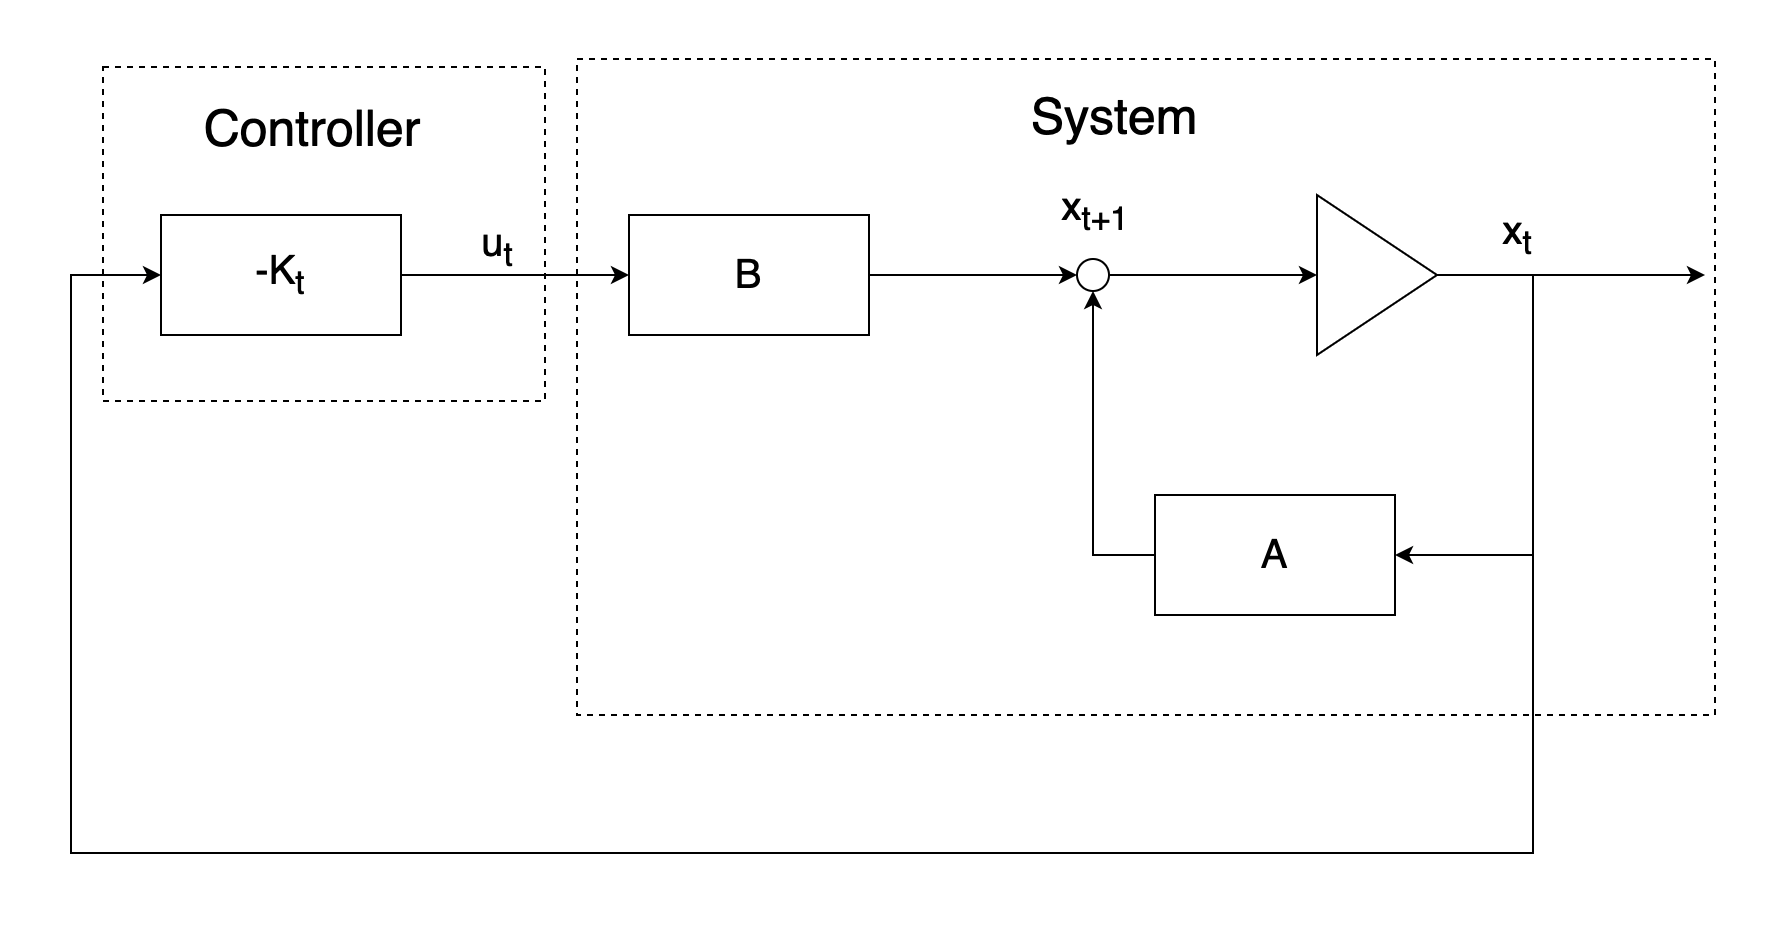
\includegraphics[width=1.0\textwidth]{../1c.png}
             \caption{The system and controller.}
             \label{fig:1c}
         \end{figure}
    \end{punkt}

    %d
    \begin{punkt}
        To solve the stationary Riccati equation I used the following code:
        \lstinputlisting{../task_1d.m}

        This gives that:
        \begin{align*}
            P &= \begin{bmatrix}
                4.0350 & 2.0616 \\
                2.0616 & 4.1438
            \end{bmatrix} \\
            K &= \begin{bmatrix}
                0.6514 \\ 1.3142
            \end{bmatrix} \\
            \lambda &= 0.6307 \pm 0.1628i
        \end{align*}

        The resulting system is stable if $|\text{eig}(A-BK)| < 1$. Since
        \begin{align*}
            |\lambda_1| = |\lambda_2| = \sqrt{0.6307^2 + 0.1628^2} = 0.6514 < 1,
        \end{align*}
        the closed-loop system is stable.
        \end{punkt}

    %e
    \begin{punkt}
        \label{1e}
        The closed-loop system is stable if the system $(A,B)$ is stabilizable and the system $(A,D)$ is detectable,
        where $D$ is defined by $Q=D^\top D$. The first part means that the system must be stabilizable, since we have a infinite horizon.
        The second part means hat we must be able to influence all unstable modes of the system. In order for us to influence
        all unstable modes we must be able to detect them in our objective function (through $D$).
    \end{punkt}
\end{oppgave}

%2
\begin{oppgave}

    %a
    \begin{punkt}
        The stationary one-dimensional Riccati equation is given by:
        \begin{align*}
            p &= q + ap(1+\frac{b^2p}{r})^{-1}a
        \end{align*}
        Some rest
        \begin{align*}
            p &= q + ap(1+\frac{b^2p}{r})^{-1}a \\
            p &= q + a^2p \frac{1}{1+\frac{b^2p}{r}} \\
            p s&= q + \frac{a^2pr}{r+b^2p}
        \end{align*}
        With $q=2$, $a=3$, $b=2$, $r=1$ we get:
        \begin{align*}
            p &= 2 + \frac{3^2p}{1+2^2p} \\
            p(1+4p) &=2(1+4p)+9p \\
            4p^2 - 16 -2 &= 0 \\
            \implies p &= \frac{16 \pm \sqrt{16^2-4(-2)4}}{8} = 2 \pm \frac{3}{\sqrt{2}}
        \end{align*}
        Since $p$ must be above 0 (see equation 4.32d in "Merging Optimization and Control"), we choose
        $p = 2 + \frac{3}{\sqrt{2}}$
    \end{punkt}

    %b
    \begin{punkt}
        The feedback gain is defined by:
        \begin{align*}
            k = \frac{bp}{r}(1 + \frac{b^2p}{r})^{-1}a
        \end{align*}
        Setting in all the values and $p = 2 + \frac{3}{\sqrt{2}}$ gives us:
        \begin{align*}
            k = \sqrt{2}
        \end{align*}
        This gives us that the optimal control law is given by:
        \begin{align*}
            u_t = -\sqrt{2}x_t
        \end{align*}
    \end{punkt}

    %c
    \begin{punkt}
        Same answer as Task \hyperref[1e]{1e}.
    \end{punkt}
\end{oppgave}

% 3
\begin{oppgave}

    % a
    \begin{punkt}
        \label{3a}
        The result from the previous assignment are shown in Figure \ref{fig:3a}.

        \begin{figure}[H]
            \centering
            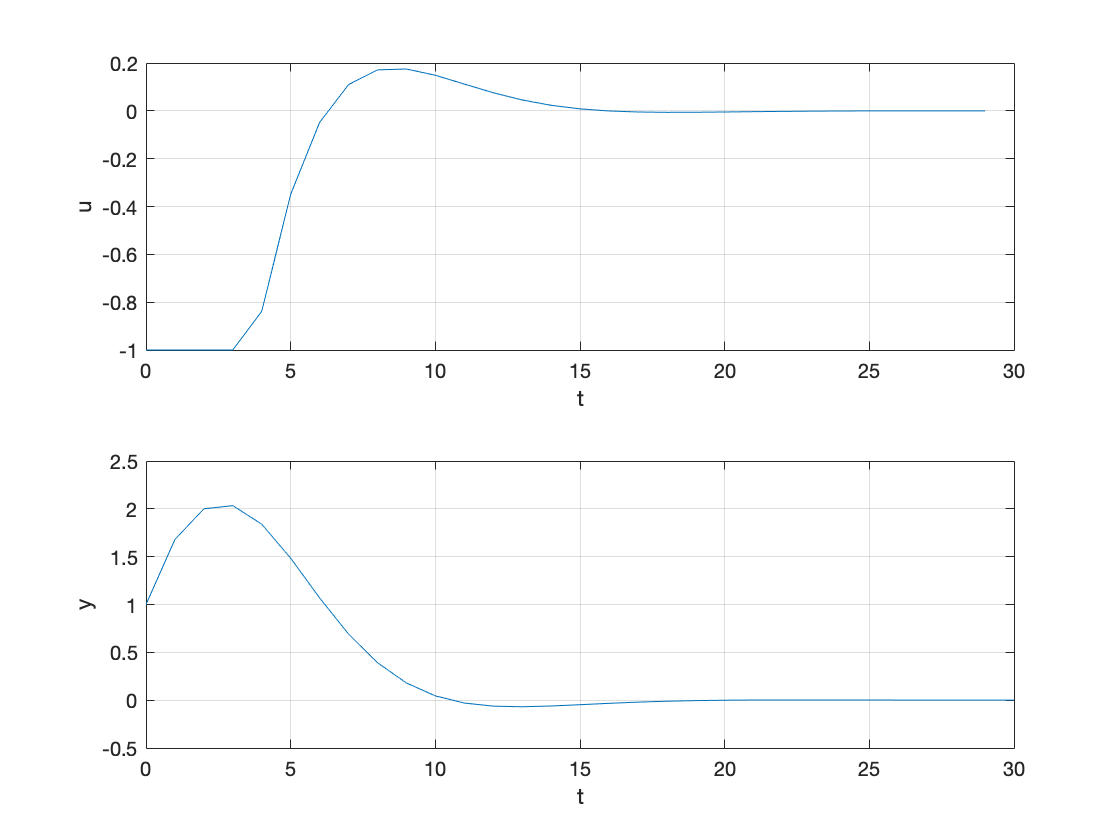
\includegraphics[width=0.8\textwidth]{../3a.png}
            \caption{$u_t$ and $y_t$ for inequality constrained control input.}
            \label{fig:3a}
        \end{figure}
    \end{punkt}

    % b
    \begin{punkt}
        Our $z$ will now only have $N/6$ control inputs. These control inputs are repeated for
        $n=5$ time steps each, so we will have the same control input for 5 rows each in $A_{eq}$. The right part of $A_{eq}$ will then have the following structure
        (simplified by just showing the row for $u_0$ and $u_1$):
        \begin{align*}
            \begin{bmatrix}
                -B & 0 & 0 & 0 & 0 & 0 \\
                -B & 0 & 0 & 0 & 0 & 0 \\
                -B & 0 & 0 & 0 & 0 & 0 \\
                -B & 0 & 0 & 0 & 0 & 0 \\
                -B & 0 & 0 & 0 & 0 & 0 \\
                -B & 0 & 0 & 0 & 0 & 0 \\
                0 & -B & 0 & 0 & 0 & 0 \\
                0 & -B & 0 & 0 & 0 & 0 \\
                0 & -B & 0 & 0 & 0 & 0 \\
                0 & -B & 0 & 0 & 0 & 0 \\
                0 & -B & 0 & 0 & 0 & 0 \\
                0 & -B & 0 & 0 & 0 & 0
            \end{bmatrix}
        \end{align*}

        Simplifying by using $\bar{B} = \begin{bmatrix}
            -B \\
            -B \\
            -B \\
            -B \\
            -B \\
            -B
        \end{bmatrix}$ gives us the following $A_{eq}$ matrix:

        \begin{align*}
            A_{eq} &= \begin{bmatrix}
                I & 0 & \dots &  \dots & 0 & -\bar{B} & 0 & \dots & \dots & 0 \\
                -A & I & \ddots &  & \vdots & 0 & \ddots & \ddots & & \vdots \\
                0 & -A & \ddots & \ddots & \vdots & 0 & \ddots & \ddots & \ddots & \vdots \\
                \vdots &  & \ddots & \ddots & 0 & \vdots &  & \ddots & \ddots & 0 \\
                0 & \dots & 0 & -A & I & 0 & \dots & \dots & 0 & -\bar{B}
            \end{bmatrix}
        \end{align*}

        The right part will now only have 6 columns due to the reduced number of control inputs.

        The modified matrices can be found in the file \texttt{task\_3b.m}.

        The results using input plotting can be found in Figure \ref{fig:3b}. As we can see the control inputs
        are repeated for 5 time steps each. The resulting $y$ graph is almost the same as the one in \hyperref[3a]{Task 3a}, even
        though we are input blocking and therefore have a smaller $z$ vector.


        \begin{figure}[H]
            \centering
            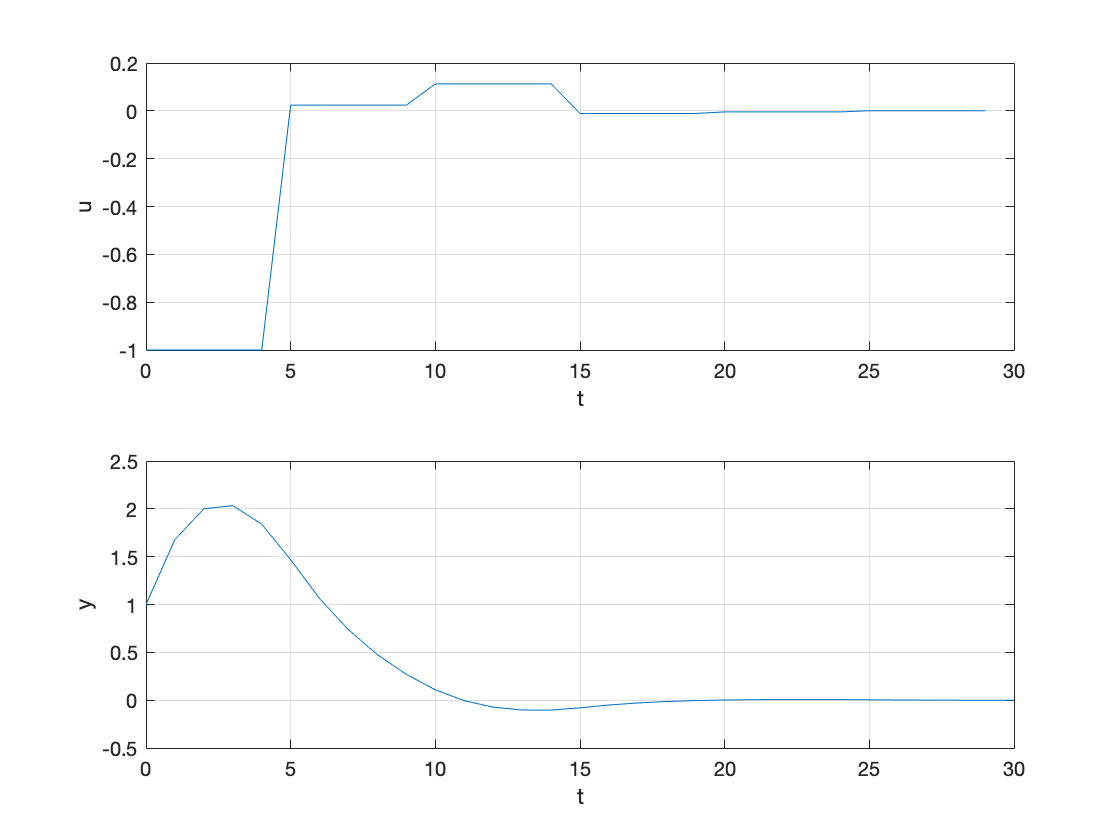
\includegraphics[width=0.8\textwidth]{../3b.png}
            \caption{$u_t$ and $y_t$ for even input blocking scheme.}
            \label{fig:3b}
        \end{figure}

        \texttt{quadprog} still used 5 iterations with the interior-point-convex method which is the same same as
        without input blocking. However when using the active-set method it went down from 5 iterations to 2. As we can see
        the choice of method used influence the results a lot.
    \end{punkt}

    % c
    \begin{punkt}
        The results using better input parametrization are found in Figure \ref{fig:3c}
        \begin{figure}[H]
            \centering
            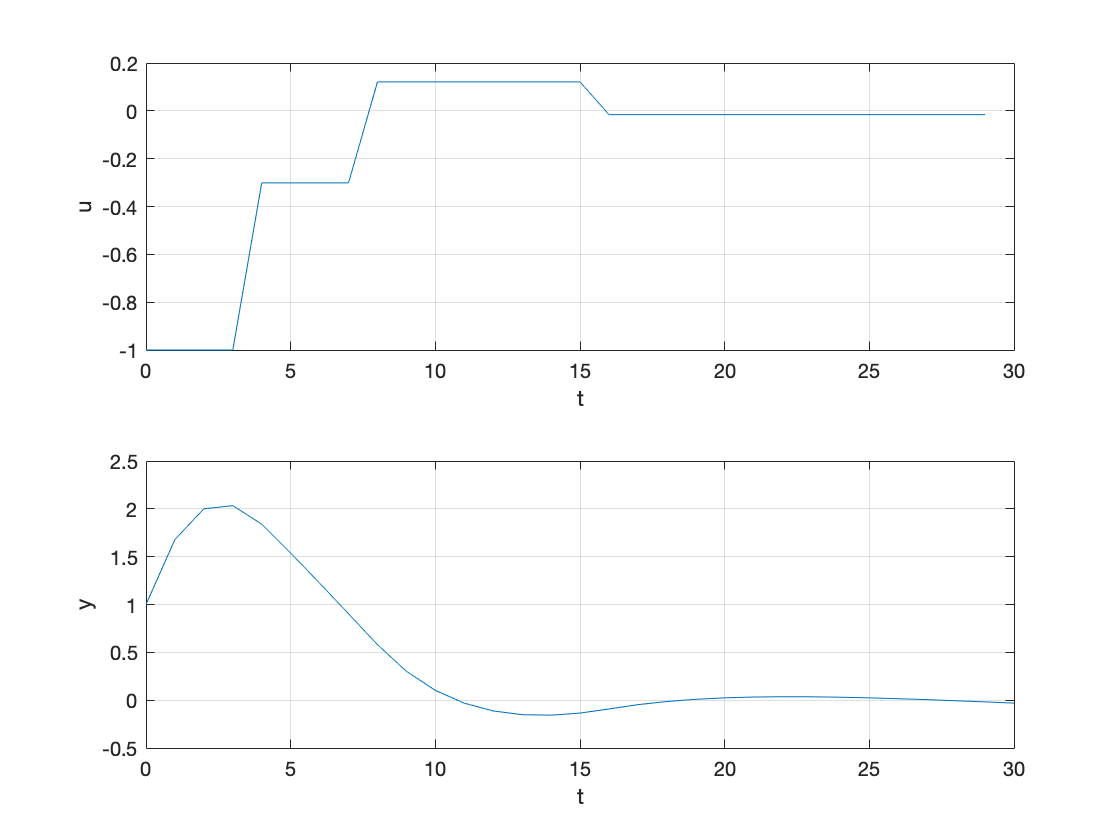
\includegraphics[width=0.8\textwidth]{../3c.png}
            \caption{$u_t$ and $y_t$ for parametrized input blocking scheme.}
            \label{fig:3c}
        \end{figure}

        As we can see the results are pretty much the same. Even though we have given the controller
        more freedom in the beginning, this doesn't really matter as the control input is at the limit -1 anyways.

        We still get 5 iterations using the interior-point-convex method.

    \end{punkt}

    % d
    \begin{punkt}
        The results from the previous assignment are shown in Figure \ref{fig:3d}.

        \begin{figure}[H]
            \centering
            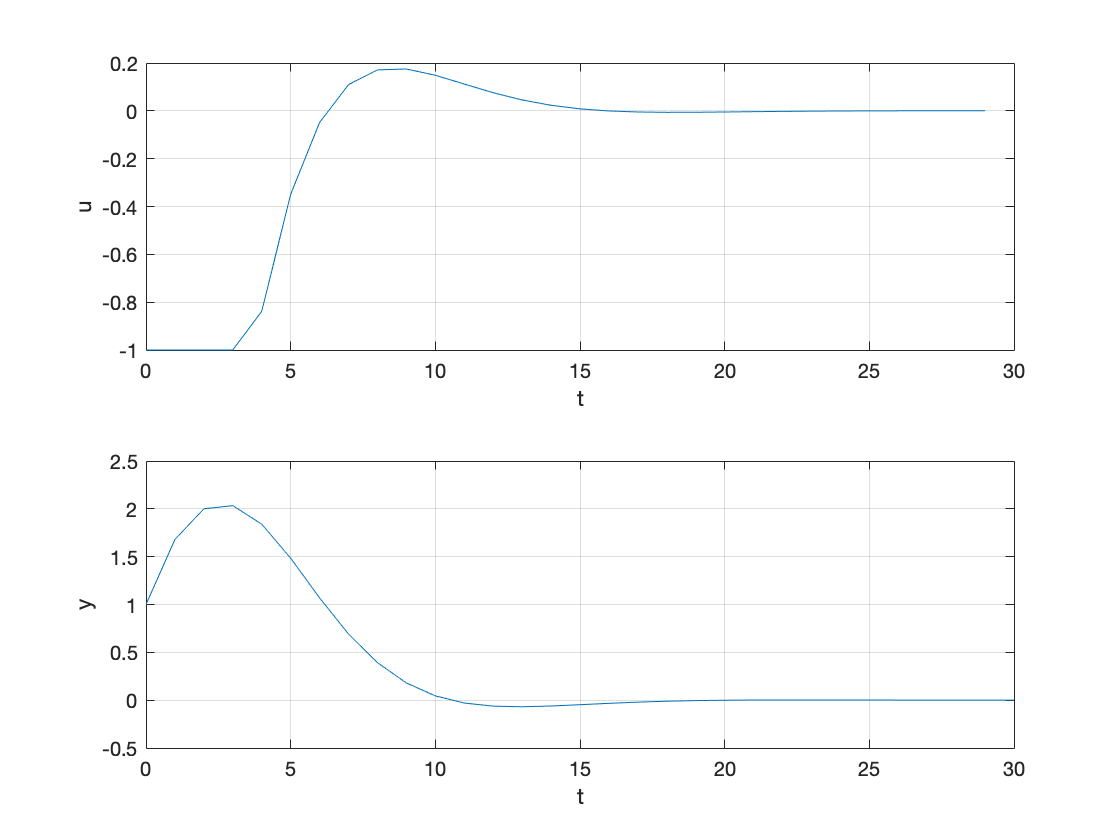
\includegraphics[width=0.8\textwidth]{../3d.png}
            \caption{$u_t$ and $y_t$ for MPC with horizon of $n=30$ with no input blocking.}
            \label{fig:3d}
        \end{figure}
    \end{punkt}

    % e
    \begin{punkt}
        The results with input blocking in MPC are shown in Figure \ref{fig:3e}.
        As we can see the difference is neglectable between the MPC with no input blocking and
        the MPC with input blocking.

        Using the interior-point-convex method the performance gain was neglectable, but
        with active-set method this performance gain was pretty significant, especially
        since we solve the optimization problem at each step.

        \begin{figure}[H]
            \centering
            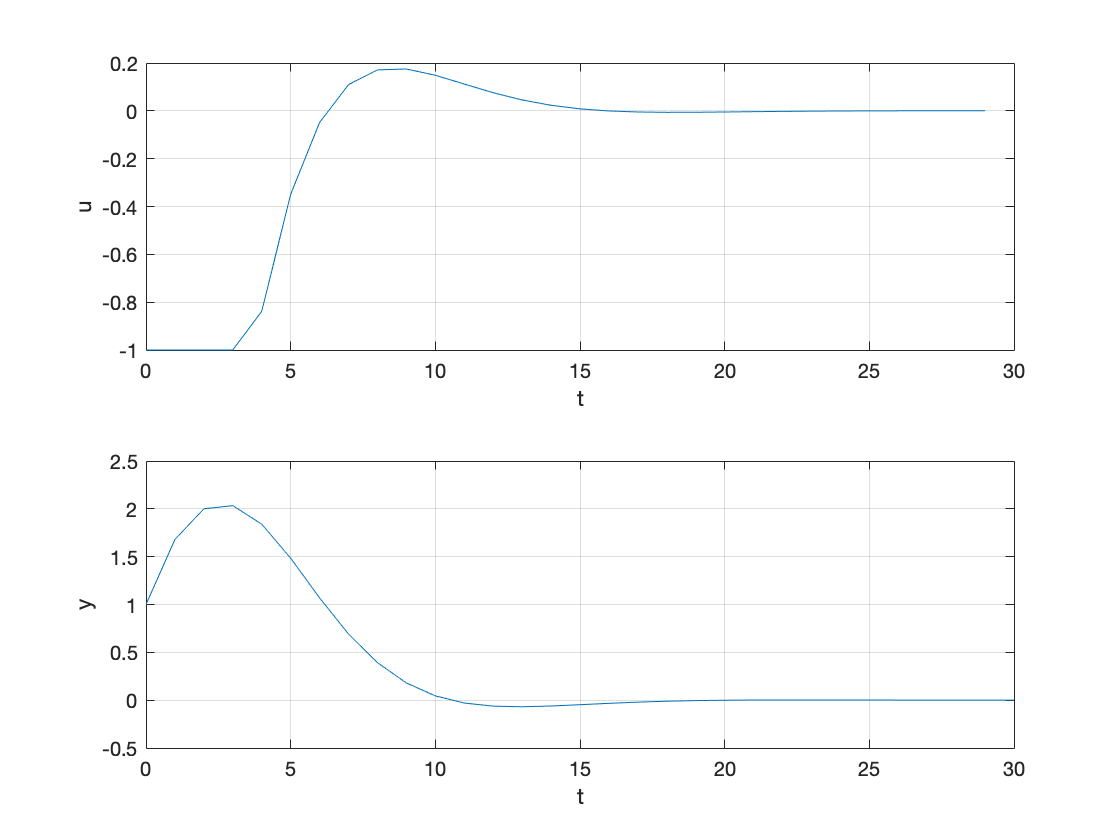
\includegraphics[width=0.8\textwidth]{../3d.png}
            \caption{$u_t$ and $y_t$ for MPC with horizon of $n=30$ with input blocking.}
            \label{fig:3e}
        \end{figure}
    \end{punkt}

    % f
    \begin{punkt}
        The effect of using input blocking is that we allow for fewer control inputs, which leads to smaller
        dimensions in the matrices used in constraints, objective function etc. Using the
        interior-point-convex method this performance gain was neglectable in this particular
        problem formulation, but with active-set method the decrease of iterations could be significant
        given that in MPC the optimization problem is solved at each time step.

        The reason for choosing input blocks of increasing length is to allow for the controller to make larger adjustments in the initial more
        unstable phase and when it goes towards a steady-state it can keep the same control input for longer.

    \end{punkt}


\end{oppgave}

\end{document}
